\documentclass[12pt]{article}
\usepackage[utf8]{inputenc}
\usepackage[english]{babel}
%\usepackage{times}
\usepackage[none]{hyphenat} % turns off word hyphenation
%\usepackage{titling}
\usepackage{hyperref}
\usepackage{fancyhdr}
\usepackage{geometry}
\usepackage{caption}
\usepackage{subcaption}
\usepackage{amsmath}
\usepackage{amssymb}
\usepackage{amsfonts}
\usepackage{mathtools}
\usepackage{graphicx}
\usepackage{float}
\usepackage{wrapfig}
\usepackage{tabularx}
\usepackage{multirow}

%\spacedforallowdisplaybreaks
\graphicspath{{./images/}}
\geometry{margin=1.2in}
\renewcommand{\baselinestretch}{1.5}
\newcommand{\spacedforall}{\;\forall\;}
\newcommand{\numberthis}{\addtocounter{equation}{1}\tag{\theequation}}
\addto\captionsenglish{\renewcommand{\contentsname}{Units}} % Change TOC title

\newcommand{\fline}{\par\noindent\rule{\textwidth}{0.1pt}} % horizontal line (wide)
\newcommand{\R}{\mathbb{R}} % symbol for real numbers

\title{High School Calculus Notes}
\author{Bryan Deng}

\begin{document}
\maketitle
\newpage
\tableofcontents
\newpage

\section{Limits and Continuity}
A limit is when a function approaches, or gets infinitely close to a value. The standard notation for a limit is:
\[ \lim_{x \to c} f(x), \]
where $x$ approaches the value $c$ from both the left (negative values) or right (positive values).

\subsection{Sided Limits}
By adding a sign superscript to the $c$, it symbolizes that $x$ can only approach from the respective direction. A right-hand limit is when $x$ approaches $c$ from values greater than $c$:
\[ \lim_{x \to c^+} f(x). \]
Similarly, a left-hand limit is when $x$ approaches $c$ from values less than $c$:
\[ \lim_{x \to c^-} f(x). \]

It is important to note that a sided limit only exists if the function itself exists on that side of the value. More specifically,
$\lim \limits_{x \to c^+} f(x)$ only exists given $f(x) \in \R \spacedforall x > c$, and $\lim \limits_{x \to c^-} f(x)$ only exists given $f(x) \in \R \spacedforall x < c$. An example of this is:
\[ \lim_{x \to 0^-} \sqrt{x} = \text{undef} \]
because the function $\sqrt{x}$ does not exist for $x < 0$.

\subsection{Limits to Infinity}
If a degree of a polynomial is greater than or equal to $1$, its limit as $x$ approaches $\pm \infty$ will also be $\pm \infty$. The limit depends on the sign of the leading coefficient and the degree of the polynomial. For example:
\begin{align*}
	\lim_{x \to \infty} 2 x^3 - 7x^2 + 2 &= \infty   \\
	\lim_{x \to -\infty} 2 x^3 - 7x^2 + 2 &= -\infty.
\end{align*}
Here, the degree of the polynomial is $3$, and the leading coefficient, $2$, is positive. The function generally increases as $x$ increases.

When dealing with fractions of polynomials, if the degree of the numerator is greater than that of the denominator, the limit will be $\pm \infty$. In order to determine the sign of the limit, subtract the degree of the denominator from that of the numerator. For example,
\begin{align*}
	\lim_{x \to \infty} \frac{x^3 + 5}{x - 2} &= \infty   \\
	\lim_{x \to -\infty} \frac{3x^2 - 3}{x + 1} &= -\infty.
\end{align*}
When the degree of the denominator is higher than that of the numerator, the limit is always $0$. Methods for when the degrees are the same will be discussed later.

\subsection{Asymptotes}
\begin{figure}[H]
	\begin{center}
		\frame{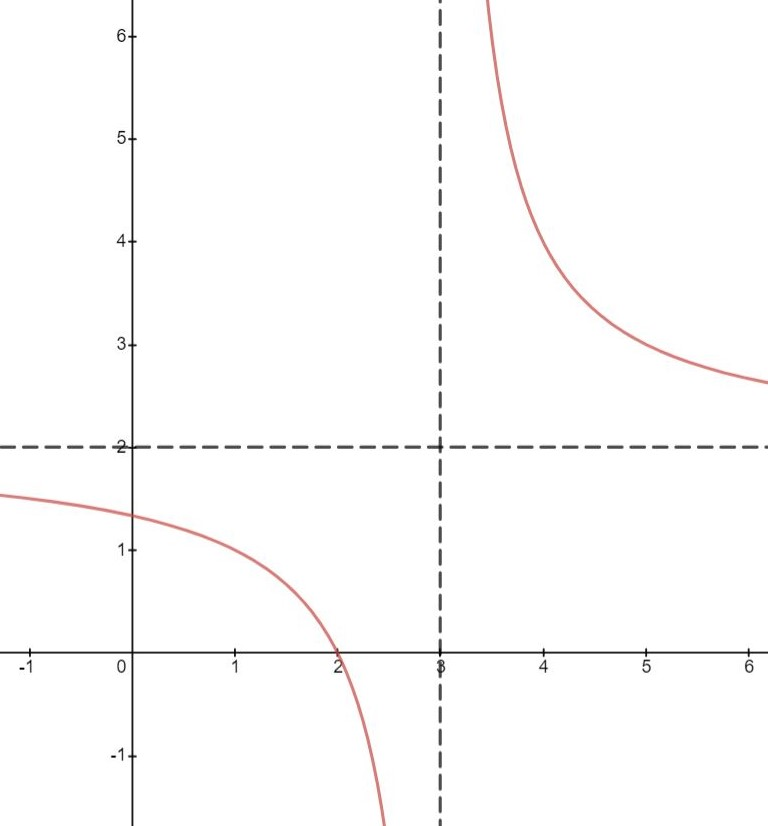
\includegraphics[width=0.5\textwidth]{fig1.JPG}}
		\caption{A function with horizontal and vertical asymptotes.}
		\label{fig:limasymptote}
	\end{center}
\end{figure}

When functions have vertical asymptotes, the limit as $x$ approaches it would be either $\infty$ or $-\infty$. It can also be undefined if the right and left sided limits have opposite signs. For example, given the function in Figure \ref{fig:limasymptote}:
\[ f(x) = \frac{2x-4}{x-3}, \]
its limits as $x \to 3$ are as follows:
\begin{align*}
	\lim_{x \to 3} & f(x) = \text{undef} \\
	\lim_{x \to 3^-} & f(x) = -\infty      \\
	\lim_{x \to 3^+} & f(x) = \infty
\end{align*}

As with horizontal asymptotes, as $x$ approaches $\pm \infty$, the function eventually gets very close to the value of the asymptote. Although the function, by definition, never touches the asymptote, the limit is equal to the $y$ value of the asymptote. Therefore:
\begin{align*}
	\lim_{x \to \infty} & f(x) = 2 \\
	\lim_{x \to -\infty} & f(x) = 2
\end{align*}

\subsection{Limit Properties}
\begin{figure}[H]
	\begin{center}
		\frame{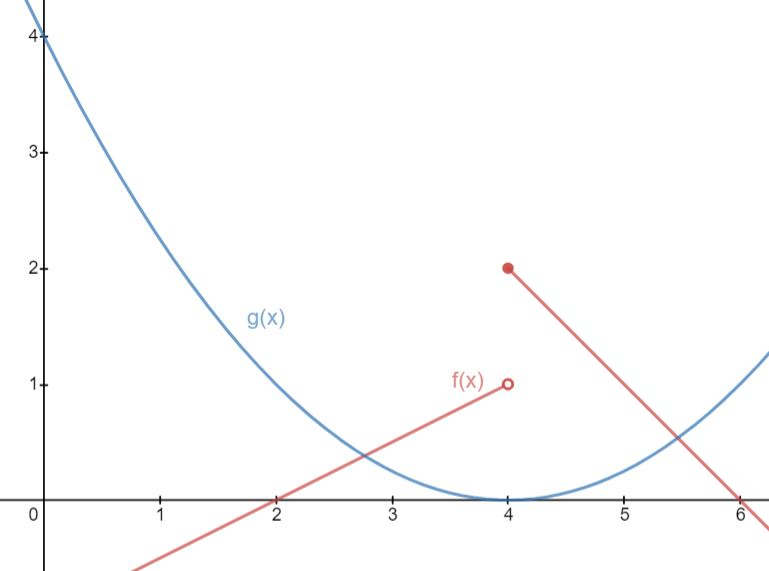
\includegraphics[scale=0.5]{fig2.JPG}}
		\caption{Two functions, $f(x)$ and $g(x)$.}
		\label{fig:limproperties}
	\end{center}
\end{figure}

Several rules can be applied when finding the limit of combined functions. The following examples are all based on Figure \ref{fig:limproperties}.

\subsubsection{Addition and Subtraction}
The combined limit of the sum or difference of two functions is equivalent to the sum or difference of the separate limits. In other words:
\[ \lim_{x \to c} \left[ f(x) \pm g(x) \right] = \lim_{x \to c} f(x) \pm \lim_{x \to c} g(x). \]
Applying this rule to the two functions in Figure \ref{fig:limproperties}:
\begin{align*}
	\lim_{x \to 2} \left[ f(x) + g(x) \right] &= \lim_{x \to 2} f(x) + \lim_{x \to 2} g(x) \\
	&= 0 + 1 \\
	\lim_{x \to 2} \left[ f(x) + g(x) \right] &= 1 \\[10pt]
	\lim_{x \to 2} \left[ g(x) - f(x) \right] &= \lim_{x \to 2} g(x) - \lim_{x \to 2} f(x) \\
	&= 1 - 0 \\
	\lim_{x \to 2} \left[ g(x) - f(x) \right] &= 1 \\[10pt]
	\lim_{x \to 4} \left[ f(x) + g(x) \right] &= \lim_{x \to 4} f(x) + \lim_{x \to 4} g(x) \\
	&= \text{undef} + 0 \\
	&= \text{undef}
\end{align*}

Note that in the last example, because the right and left side limits of $f(x)$ are not the same, its limit at $x = 4$ is \textit{undefined}. When adding $f(x)$ and $g(x)$, if just one of the functions has an undefined limit, the combined limit would also be undefined.

A generalization of the addition and subtraction properties for more than two functions is defined by the \textit{extended sum rule}. It states that:
\[ \lim_{x \to c} \left[ \sum_i f_i(x) \right] = \sum_i \left[ \lim_{x \to c} f_i(x) \right]. \]
Or in expanded notation:
\[ \lim_{x \to c} \left[ f_1(x) + \cdots + f_n(x) \right] = \lim_{x \to c} f_1(x) + \cdots + \lim_{x \to c} f_n(x). \]

\subsubsection{Multiplication}
Similar to addition and subtraction, the product of two functions is equivalent to the product of the separate limits. In other words:
\[ \lim_{x \to c} \left[ f(x) g(x) \right] = \lim_{x \to c} f(x) \lim_{x \to c} g(x). \]
Applying this rule to the two functions in Figure \ref{fig:limproperties}:
\begin{align*}
	\lim_{x \to 2} \left[ f(x) g(x) \right]
	&= \lim_{x \to 2} f(x) \cdot \lim_{x \to 2} g(x) \\
	&= 0 \cdot 2 \\
	&= 0
\end{align*}
The same exception applies when one of the limits is \textit{undefined}. This just makes the entire product's limit undefined.

A generalization of the product rule for more than two functions is defined by the \textit{extended product rule}, and is quite similar to the extended sum rule. It states that:
\[ \lim_{x \to c} \left[ \prod_i f_i(x) \right] = \prod_i \left[ \lim_{x \to c} f_i(x) \right]. \]
Or in expanded notation:
\[ \lim_{x \to c} \left[ f_1(x) f_2(x) \cdots f_n(x) \right] = \lim_{x \to c} f_1(x) \times \lim_{x \to c} f_2(x) \cdots \lim_{x \to c} f_n(x). \]

\subsubsection{Division}
In similar fashion, the quotient of two functions is equivalent to the quotient of the separate limits, as long as the limit of the denominator is not $0$. In other words:
\[ \lim_{x \to c} \frac{f(x)}{g(x)} = \frac{\lim_{x \to c} f(x)}{\lim_{x \to c} g(x)} \Rightarrow \lim_{x \to c} g(x) \ne 0. \]
Applying this rule to the two functions in Figure \ref{fig:limproperties}:
\begin{align*}
	\lim_{x \to 2} \frac{g(x)}{f(x)} &= \frac{\lim_{x \to 2} g(x)}{\lim_{x \to 2} f(x)} \\
	&= \frac{1}{0} \\
	&= \text{undef}
\end{align*}

\subsubsection{Composite Functions}
When finding the limit of a composite function, such as $f\left( g(x) \right)$, first evaluate the limit of the inner function, then evaluate the outer function normally. Hence:
\[ \lim_{x \to c} f\left( g(x) \right) = f\left( \lim_{x \to c} g(x) \right). \]
Applying this rule to the two functions in Figure \ref{fig:limproperties}:
\begin{align*}
	\lim_{x \to 1} f\left( g(x) \right) &= f\left( \lim_{x \to 1} g(x) \right) \\
	&= f(2) \\
	&= 0
\end{align*}
When the limit of the inner function is undefined, the limit of the composite equation would also be undefined. This is because the outer function does not exist at an undefined point.
\begin{align*}
	\lim_{x \to 4} g\left( f(x) \right) &= g\left( \lim_{x \to 4} f(x) \right) \\
	&= g(\text{undef}) \\
	&= \text{undef}
\end{align*}

\subsubsection{Constants}
Given that $\lim \limits_{x \to c} f(x)$ and $\lim \limits_{x \to c} g(x)$ are both finite for all $c \in \R$, then the following two equations hold:
\begin{gather*}
	\lim_{x \to c} k f(x) = k \lim_{x \to c} f(x) \\
	\lim_{x \to c} A = A
\end{gather*}
where $k$ and $A$ are both constants.

\subsection{Solving Limits}
There are several methods that can be used to solve a limit depending on various outcomes such as undefined solutions or indeterminate forms. These are outlined below.

\subsubsection{Direct Substitution}
The first method to try when solving a limit is \textbf{direct substitution}. For example:
\[ \lim_{x \to 6} -x^2 = -6^2 = -36. \]

There are two cases for when direct substitution will not work. The first of which is when it results in an undefined solution in the form $\frac{k}{0}$, where $k \in \R$. This means that there is likely an asymptote, and further methods can be used to determine a definite solution. The second of which is in the form $\frac{0}{0}$, which is called an \textit{indeterminate form}. This can be solved using either algebraic manipulation or L'Hopital's rule, to be mentioned later.

\subsubsection{Algebraic Manipulation}
When direct substitution results in an undefined value, the next method to try is algebraic manipulation. Such a method can involve factoring or polynomial division. For example:
\begin{align*}
	\lim_{x \to 2} \frac{x^4 + 3x^3 - 10x^2}{x^2 - 2x} & = \lim_{x \to 2} \frac{x^2 (x + 5)(x - 2)}{x(x - 2)} \\[5pt]
	&= \lim_{x \to 2} x(x + 5) \\
	&= 14
\end{align*}

However, not all functions can be factored. In these cases, if direct substitution does not work, the limit will evaluate to be undefined. For example:
\begin{align*}
	\lim_{x \to 1} \frac{2x}{x^2 - 7x + 6} &= \lim_{x \to 1} \frac{2x}{(x-6)(x-1)} \\
	&= \frac{2}{0} \\
	&= \text{undef}
\end{align*}

\subsubsection{Trigonometric Identities}
Trig identities can be used when dealing with trig equations, and direct substitution does not work. It will be useful to know the basic identities, among other ones:
\begin{table}[H]
	\centering
	\begin{tabular}{|c|c|}
		\hline
		\textbf{Pythagorean's identity} & $\sin^2(x) + \cos^2(x) = 1$ \\
		\hline
		\multirow{4}{*}{\textbf{Double angle identities}} & $\sin(2x) = 2 \sin(x) \cos(x)$ \\
		& $\cos(2x) = \cos^2(x) - \sin^2(x)$ \\
		& $\cos(2x) = 2\cos^2(x) - 1$ \\
		& $\cos(2x) = 1 - 2\sin^2(x)$ \\
		\hline
		\multirow{3}{*}{\textbf{Reciprocal identities}} & $\csc(x) = \frac{1}{\sin(x)}$ \\[5pt]
		& $\sec(x) = \frac{1}{\cos(x)}$ \\[5pt]
		& $\cot(x) = \frac{1}{\tan(x)} = \frac{\cos(x)}{\sin(x)}$ \\[5pt]
		\hline
	\end{tabular}
\end{table}

An example of when trig identities can be used to solve a limit is the limit as $x \to \frac{\pi}{2}$ for the function $f(x) = \frac{\cot^2(x)}{1 - \sin(x)}$. If direct substitution is used, it results in an indeterminate form $\frac{0}{0}$. Therefore, the limit can be solved as follows:
\begin{align*}
	\lim_{x \to \frac{\pi}{2}} \frac{\cot^2(x)}{1 - \sin(x)} &= \lim_{x \to \frac{\pi}{2}} \frac{1}{1 - \sin(x)} \left( \frac{\cos(x)}{\sin(x)} \right)^2 \\[5pt]
	&= \lim_{x \to \frac{\pi}{2}} \frac{\cos^2(x)}{\sin^2(x) (1 - \sin(x))} \\[5pt]
	&= \lim_{x \to \frac{\pi}{2}} \frac{1 - \sin^2(x)}{\sin^2(x) (1 - \sin(x))} \\[5pt]
	&= \lim_{x \to \frac{\pi}{2}} \frac{(1 + \sin(x))(1 - \sin(x))}{\sin^2(x) (1 - \sin(x))} \\[5pt]
	&= \lim_{x \to \frac{\pi}{2}} \frac{1 + \sin(x)}{\sin^2(x)} , \, 1 - \sin(x) \ne 0 \\[5pt]
	&= 2
\end{align*}

\subsection{Continuity}
A function is continuous $f(x)$ is continuous at a point $x = c$ if:
\[ \lim_{x \to c} f(x) = f(c). \] % the definition for continuity in the previous version was faulty

A function is continuous over the interval $[a, b]$ if it is continuous at each point within the interval. Some examples of functions and the intervals for which they are continuous:
\begin{itemize}
	\item $\sqrt{x + 4}$ is continuous for all $x \in [-4, \infty)$.
	\item $\sqrt[5]{x}$ is continuous for all $x \in \R$.
	\item $\ln x$ is continuous for all $x \in [0, \infty)$.
	\item $\frac{1}{x - 3}$ is continuous for all $x \ne 3$.
\end{itemize}

In general, functions won't be continuous if they have a division by $0$, square root of a negative number, or logarithm of $0$. For example, find the values of $x$ for which $f(x) = \frac{3x + 4}{x^2 - 3x + 2}$ is not continuous. In this function, $f(x)$ is undefined if the denominator is $0$, therefore it is not continuous for when:
\begin{align*}
	x^2 - 3x + 2 &= 0 \\
	(x - 2)(x - 1) &= 0 \\
	x &= 1, \, 2
\end{align*}
Altogether, the function $f(x)$ is continuous for $x \in \R, x \ne 1, \, 2$.

\subsubsection{Removable Discontinuity}
A function has a point of removable discontinuity if the value at that point is either undefined, or different from the limit of the function at that point. A function $f(x)$ has removable discontinuity at a point $x = c$ if:
\[ f(x) = \begin{cases}
		g(x) & \text{if} \; x \ne c \\
		k    & \text{if} \; x = c
	\end{cases} \quad \text{where} \, \lim_{x \to c} f(x) = g(c).\]

An example of a function with removable discontinuity is the function $f(x) = \frac{x - 2}{x - 2}$. This function is undefined at $x = 2$, but resembles the function $y = 1$ everywhere else. It can therefore be rewritten as:
\[ f(x) = \begin{cases}
    1 & \text{if} \; x \ne 2 \\
    \text{undef} & \text{if} \; x = 2
\end{cases}. \]
Notice that the limit of $f(x)$ as $x$ approaches $2$ is equal to $1$. Hence, the function has removable discontinuity at $x = 2$.

\subsubsection{Jump Discontinuity}
A function has a point of jump discontinuity if that part of the graph ``jumps'' from one $y$ value to another on the same $x$. The sided limits of the function at the point $x$ both exist, but are not equal. For example, function $f(x)$ from \ref{fig:limproperties} has jump discontinuity at $x = 4$. It can be denoted as follows:
\[ f(x) = \begin{cases}
    \frac{x}{2} - 1 & \text{if} \; x < 4 \\
    -x + 6 & \text{if} \; x \ge 4
\end{cases}. \]

\subsubsection{Infinite Discontinuity}
A function has a point of infinite discontinuity if the $y$ value at a point $x$ approaches $\pm \infty$. This usually happens at a vertical asymptote. The sided limits both exist, and both approach $\pm \infty$. For example, the function $f(x) = \frac{1}{x}$ has infinite discontinuity at $x = 0$. This can be verified by:
\[ \lim_{x \to 0^-} f(x) = -\infty \quad \text{and} \quad \lim_{x \to 0^+} f(x) = \infty. \]

\subsection{Squeeze Theorem}
The squeeze theorem, also known as the sandwich theorem, can be used to find the limit of a function at a particular value, especially when direct evaluation of the limit is difficult.

Given an open interval $I$ that includes a point $c$, where all points, and three functions within the interval such that:
\[ f(x) \le g(x) \le h(x), \]
for every $x$ in $I$ not equal to $c$, and that:
\[ \lim_{x \to c} f(x) = \lim_{x \to c} h(x) = L, \]
then $\lim \limits_{x \to c} g(x) = L$.

\noindent \textbf{Examples:}
\begin{enumerate}
    \item Find $\lim \limits_{x \to \infty} \frac{\sin x}{x}$.

    First, set up an inequality with the simpler part of the function, $\sin x$. The range of the $\sin x$ function is $[-1, 1]$. Therefore:
    \[ -1 \le \sin x \le 1. \]
    Next, divide the inequality by $x$ to resemble the original function:
    \[ -\frac{1}{x} \le \frac{\sin x}{x} \le \frac{1}{x}. \]
    Since $\lim \limits_{x \to \infty} -\frac{1}{x} = \lim \limits_{x \to \infty} \frac{1}{x} = 0$, by the squeeze theorem, $\lim \limits_{x \to \infty} \frac{\sin x}{x}$ must also be $0$. Therefore:
    \[ \lim \limits_{x \to \infty} \frac{\sin x}{x} = 0. \]

    \item Find $\lim \limits_{x \to -\infty} \frac{x^2 (\sin x + \cos^3 x)}{(x^2 + 1)(x - 3)}$.

	The part of this function that is most likely to have a range is $\sin x + \cos^3 x$. The ranges of $\sin x$ and $\cos x$ are both $[-1, 1]$. Therefore:
	\begin{gather*}
		-1 \le \sin x \le 1 \numberthis{\label{eq:sin_range}} \\
		-1 \le \cos x \le 1
	\end{gather*}
	Taking the cube of the second inequality:
	\[ -1 \le \cos^3 x \le 1 \numberthis{\label{eq:cos3_range}}. \]
	Adding inequalities \eqref{eq:sin_range} and \eqref{eq:cos3_range} gets the range of part of the numerator of the original function:
	\[ -2 \le \sin x + \cos^3 x \le 2. \]
	Next, multiply the inequality by $\frac{x^2}{(x^2 + 1)(x - 3)}$:
	\[ \frac{-2 x^2}{(x^2 + 1)(x - 3)} \le \sin x + \cos^3 x \le \frac{2 x^2}{(x^2 + 1)(x - 3)}. \]
	Since
	\[ \lim_{x \to -\infty}\frac{-2 x^2}{(x^2 + 1)(x - 3)} = 0 \quad \text{and} \quad \lim_{x \to -\infty}\frac{2 x^2}{(x^2 + 1)(x - 3)} = 0, \]
	by the squeeze theorem,
	\[ \lim_{x \to -\infty} \frac{x^2 (\sin x + \cos^3 x)}{(x^2 + 1)(x - 3)} = 0. \]
\end{enumerate}

\subsection{Intermediate Value Theorem}
Given a \textbf{continuous} segment of a function $f(x)$, let $c \in [a, b]$ and $w$ be in between $f(a)$ and $f(b)$. By the intermediate value theorem, there must be at least one value $c$ such that $f(c) = w$. That is, a continuous line in between points $A$ and $B$ must pass through every $x$ and $y$ value in between them. This goes both ways: if there is a $c$ then there is a $w$, and vice versa.

\begin{figure}[H]
	\begin{center}
		\frame{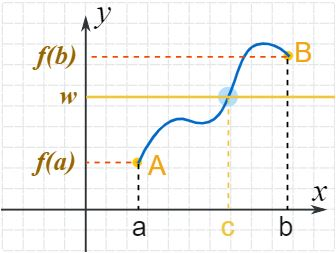
\includegraphics{images/fig3.JPG}}
	\end{center}
	\label{fig:inter_value_theorem}
	\caption{Visualization of the intermediate value theorem.}
\end{figure}

\section{Differentiation}
A derivative is the \textbf{instantaneous} rate of change of a function at a point, or the average rate of change over an infinitely small interval. There are two notations for derivatives:

\begin{itemize}
	\item \textbf{Lagrange's notation:} The derivative of $f(x)$ if $f'(x)$. The $n$-th order derivative is written as $f^n(x)$, or with $n$ ticks.
	\item \textbf{Leibniz's notation:} The derivative of $f$ is $\frac{d}{dx}$, indicating a derivative with respect to $x$. When $y = f(x)$,  the first derivative is written as $\frac{dy}{dx}$. The $n$-th order derivative is written as $\frac{d^n y}{dx^n}$.
\end{itemize}

\subsection{Continuity and Differentiability}
\textbf{Differentiability} means that the function must be differentiable for every value in its domain. On the other hand, \textbf{continuity} means that the function has no breaks over its domain, or ``can be drawn without lifting the pencil''. While differentiability implies continuity, continuity does not mean differentiability.

\subsection{Limit Definition of the Derivative}
This is also known as the first principle of derivatives. Because derivatives involve changes in slope over \textit{infinitely} small sections of a curve, it can be expressed as a limit. Given a function $f(x)$, its derivative $f'(x)$ can be written as:
\[ f'(x) = \lim_{h \to 0} \frac{f(x + h) - f(x)}{h}. \]

Notice the similarity in definition between this and that for slope of a linear line, $m = \frac{\Delta y}{\Delta x}$. The numerator, $f(x + h) - f(x)$, represents an infinitely small change in $y$, and the denominator is an infinitely small change in $x$. The first principle can also be written as:
\[ f'(a) = \lim_{x \to a} \frac{f(x) - f(a)}{x - a}. \]

\subsection{Differentiation Rules}

\subsubsection{Derivative of a Constant}
The derivative of a constant is always $0$. This is because a constant would be a horizontal line, and its rate of change (slope) is always $0$.
\begin{align*}
	f(x) &= C \\
	f'(x) &= 0
\end{align*}
For example, the derivative of $f(x) = \pi$ is $f'(x) = 0$.

\subsubsection{Power Rule}
Given a function in the form $f(x) = x^p$ such that $p \in \R$, its derivative can be found by moving $p$ in front of $x$, and subtracting one from the exponent. This also applies to negative or fractional exponents.
\begin{align*}
	f(x) &= x^p \\
	f'(x) &= px^{p - 1}
\end{align*}
For example, the derivative of $f(x) = x^{24}$ is found as follows:
\[ f'(x) = 24 x^{24 - 1} = 24x^{23}. \]
As another example, the derivative of $g(x) = \sqrt[3]{x^2}$ can be found as follows:
\begin{gather*}
	g(x) = \sqrt[3]{x^2} = x^{\frac{2}{3}} \\
	g'(x) = \frac{2 x^{\frac{2}{3} - 1}}{3} = \frac{2 x^{-\frac{1}{3}}}{3} = \frac{2}{3 \sqrt[3]{x}}.
\end{gather*}

\subsubsection{Constant Coefficient}
The constant coefficient of a function can be moved outside the derivative.
\[ \frac{d}{dx} \left( k f(x) \right) = k f'(x). \]
For example, the derivative of $f(x) = 5x^2$ can be found as follows:
\begin{align*}
	f'(x) &= \frac{d}{dx} \left( 5x^2 \right) \\[5pt]
	&= 5 \left( \frac{d}{dx} \left( x^2 \right) \right) \\
	&= 5 \cdot 2x \\
	f'(x) &= 10x
\end{align*}

\subsubsection{Sum Rule}
The derivative of the sum of several functions is equal to the sum of the derivative of the individual functions. The same applies for subtraction.
\[ \frac{d}{dx} \left( \sum_i f_i(x) \right) = \sum_i f_i'(x). \]
Or in expanded form:
\[ \frac{d}{dx} \left( f_1(x) + f_2(x) + \cdots + f_n(x) \right) = f_1'(x) + f_2'(x) + \cdots + f_n'(x). \]
For example, the derivative of $f(x) = x^3 + x$ can be found as follows:
\begin{align*}
	f'(x) &= \frac{d}{dx} \left( x^3 + x \right) \\[5pt]
	&= \frac{d}{dx} \left( x^3 \right) + \frac{d}{dx} (x) \\[5pt]
	f'(x) &= 3x^2 + 1
\end{align*}

\subsubsection{Product Rule}
The derivative of the product of two functions is given by:
\[ \frac{d}{dx} \left[ f(x) g(x) \right] = f(x) g'(x) + f'(x) g(x). \]
For example, the derivative of $f(x) = x^2 e^x$ can be found as follows (the derivative of $e^x$ is explained in \ref{sec:deriv_exp_funcs}):
\begin{align*}
	f'(x) &= \frac{d}{dx} \left( x^2 e^x \right) \\[5pt]
	&= x^2 \cdot \frac{d}{dx} \left( e^x \right) + \frac{d}{dx} \left( x^2 \right) \cdot e^x \\[5pt]
	f'(x) &= x^2 e^x + 2x e^x
\end{align*}

\subsubsection{Quotient Rule}
The derivative of one function divided by another function is given by the formula below. It may be helpful to realize the similarities between the quotient and product rules for memorization.
\[ \frac{d}{dx} \left( \frac{f(x)}{g(x)} \right) = \frac{f'(x) g(x) - f(x) g'(x)}{g(x)^2}. \]
For example, the derivative of $f(x) = \frac{x^3}{e^x}$ can be found as follows (the derivative of $e^x$ is explained in \ref{sec:deriv_exp_funcs}):
\begin{align*}
	f'(x) &= \frac{d}{dx} \left( \frac{x^3}{e^x} \right) \\[5pt]
	&= \frac{\frac{d}{dx} \left( x^3 \right) \cdot e^x - x^3 \cdot \frac{d}{dx} \left( e^x \right)}{\left( e^x \right)^2} \\[5pt]
	&= \frac{3x^2 e^x - x^3 e^x}{e^{2x}} \\[5pt]
	f'(x) &= \frac{3x^2 - x^3}{e^x}
\end{align*}

\subsubsection{Chain Rule}
The chain rule allows for the differentiation of a composition of two or more functions, such as $f(g(x))$. The formula is:
\[ \frac{d}{dx} \left[ f(g(x)) \right] = f'(g(x)) g'(x). \]
For compositions of more functions, simply apply the formula recursively:
\begin{align*}
	\frac{d}{dx} \left[ f(g(h(x))) \right] &= f'(g(h(x))) \cdot \frac{d}{dx} \left[ g(h(x)) \right] \\
	&= f'(g(h(x))) g'(h(x)) h'(x).
\end{align*}
For example, the derivative of $f(x) = \sin x^2$ can be found as follows (the derivative of $\sin x$ is explained in \ref{sec:deriv_trig_funcs}):
\begin{align*}
	f'(x) &= \frac{d}{dx} \left( \sin x^2 \right) \\[5pt]
	&= \cos x^2 \cdot 2x \\
	f'(x) &= 2x \cos x^2.
\end{align*}

\subsection{Exponential Functions}
\label{sec:deriv_exp_funcs}
The formula for finding a function in the form $f(x) = a^x$ where $a$ is a constant is:
\[ \frac{d}{dx} (a^x) = a^x \ln a. \]
If the value of the constant is $e$, the derivative works out nicely:
\[ \frac{d}{dx} (e^x) = e^x \ln e = e^x. \]

\subsection{Logarithmic Functions}
The derivative of $\ln x$ is:
\[ \frac{d}{dx} (\ln x) = \frac{1}{x}. \]
This can be used to derive the derivative of other base logarithms using the log base change formula:
\begin{align*}
	\frac{d}{dx} (\log_a x) &= \frac{d}{dx} \left( \frac{\ln x}{\ln a} \right) \\[5pt]
	&= \frac{1}{\ln a} \cdot \frac{d}{dx} (\ln x) \\[5pt]
	\frac{d}{dx} (\log_a x) &= \frac{1}{x \ln a}
\end{align*}

\subsection{Trigonometric Functions}
\label{sec:deriv_trig_funcs}
The derivatives of the common trigonometric functions are listed below:
\begin{center}
	\begin{tabular}{|c|c|}
		\hline
		$f(x)$ & $f'(x)$ \\
		\hline \hline
		$\sin{x}$ & $\cos{x}$ \\
		\hline
		$\cos{x}$ & $-\sin{x}$ \\
		\hline
		$\tan{x}$ & $\frac{1}{\cos^2{x}}$ \\
		\hline \hline
		$\cot{x}$ & $-\frac{1}{\sin^2{x}}$ \\
		\hline
		$\sec{x}$ & $\tan{x} \sec{x}$ \\
		\hline
		$\csc{x}$ & $-\cot{x} \csc{x}$ \\
		\hline
	\end{tabular}
\end{center}

\subsection{Implicit Differentiation}
Implicit different is a technique that can be used to find $\frac{dy}{dx}$ in an equation, without having to explicitly solve for $y$ in terms of $x$. Simply differentiation both sides of the equation, with respect to one of the variables. For example, differentiating the following equation:
\begin{align*}
	x^2 + y^2 &= 1 \\
	\frac{d}{dx} (x^2 + y^2) &= \frac{d}{dx} \\[5pt]
	\frac{d}{dx} (x^2) + \frac{d}{dx} (y^2) &= 0 \\[5pt]
	2x + 2y \cdot \frac{d}{dx} &= 0 \\[5pt]
	\frac{dy}{dx} &= -\frac{x}{y}
\end{align*}
Notice that when differentiating the $y$ terms, the derivative is multiplied by $\frac{dy}{dx}$, as the equation is being differentiated \textbf{as a function of $x$}. Here is a slightly more complicated example:
\begin{align*}
	\frac{y}{x} &= 7 \\[5pt]
	\frac{x \cdot \frac{dy}{dx} - y}{x^2} &= 0 \\[5pt]
	x \cdot \frac{dy}{dx} - y &= 0 \\[5pt]
	\frac{dy}{dx} &= \frac{y}{x}
\end{align*}

\subsection{Inverse Functions}
Given a function $f(x)$ such that $g(x) = f^{-1}(x)$, the derivative of $g(x)$ can be found with the following formula:
\[ g'(x) = \frac{1}{f'(g(x))}. \]
The derivation for this formula is as follows:
\begin{align*}
	g(x) &= f^{-1}(x) \\
	f(g(x)) &= f(f^{-1}(x)) \\
	f(g(x)) &= x \\
	\frac{d}{dx} \left[ f(g(x)) \right] &= \frac{d}{dx} (x) \\[5pt]
	f'(g(x)) g'(x) &= 1 \\
	g'(x) &= \frac{1}{f'(g(x))}
\end{align*}
For example, given a function $f(x) = e^x$, find the derivative of its inverse, $(f^{-1})'(x)$:
\begin{align*}
	f(x) = e^x &\Rightarrow f^{-1}(x) = \ln{x} \\
	f'(x) &= e^x \\
	(f^{-1})'(x) &= \frac{1}{f' \left( f^{-1}(x) \right)} \\[5pt]
	&= \frac{1}{f'(\ln{x})} \\[5pt]
	&= \frac{1}{f'(\ln{(1)})} \\[5pt]
	&= \frac{1}{e^{\ln{(1)}}} \\[5pt]
	&= \frac{1}{1} \\[5pt]
	(f^{-1})'(x) &= 1
\end{align*}

\subsection{Inverse Trigonometric Functions}
The derivatives of the inverse trigonometric functions are listed below:
\begin{center}
	\begin{tabular}{|c|c|}
		\hline
		$f(x)$ & $f'(x)$ \\
		\hline \hline
		$\sin^{-1} x$ & $\frac{1}{\sqrt{1-x^2}}$ \\
		\hline
		$\cos^{-1} x$ & $-\frac{1}{\sqrt{1-x^2}}$ \\
		\hline
		$\tan^{-1} x$ & $\frac{1}{1+x^2}$ \\
		\hline
	\end{tabular}
\end{center}

\subsubsection{Derivations}
\begin{itemize}
	\item Derivative of $\sin^{-1} x$:
	\begin{align*}
		y &= \sin^{-1} x \\
		\sin y &= x \\
		\frac{d}{dx} (\sin y) &= \frac{d}{dx} (x) \\[5pt]
		\cos y \cdot \frac{dy}{dx} &= 1 \\[5pt]
		\frac{dy}{dx} &= \frac{1}{\cos y} \\[5pt]
		\frac{dy}{dx} &= \frac{1}{\sqrt{\cos^2 y}} \\[5pt]
		\frac{dy}{dx} &= \frac{1}{\sqrt{ - \sin^2 y}} \\[5pt]
		\frac{dy}{dx} &= \frac{1}{\sqrt{ - x^2}}
	\end{align*}

	\item Derivative of $\cos^{-1} x$:
	\begin{align*}
		y &= \cos^{-1} x \\
		\cos y &= x \\
		\frac{d}{dx} (\cos y) &= \frac{d}{dx} (x) \\[5pt]
		-\sin y \cdot \frac{dy}{dx} &= 1 \\[5pt]
		\frac{dy}{dx} &= -\frac{1}{\sin y} \\[5pt]
		\frac{dy}{dx} &= -\frac{1}{\sqrt{\sin^2 y}} \\[5pt]
		\frac{dy}{dx} &= -\frac{1}{\sqrt{1 - \cos^2 y}} \\[5pt]
		\frac{dy}{dx} &= -\frac{1}{\sqrt{1 - x^2}}
	\end{align*}

	\item Derivative of $\tan^{-1} x$:
	\begin{align*}
		y &= \tan^{-1} x \\
		\tan y &= x \\
		\frac{d}{dx} (\tan y) &= \frac{d}{dx} (x) \\[5pt]
		\sec^2 y \cdot \frac{dy}{dx} &= 1\\[5pt]
		\frac{dy}{dx} &= \cos^2 y \\[5pt]
		\frac{dy}{dx} &= \frac{\cos^2 y}{\cos^2 y + \sin^2 y} \\[5pt]
		\frac{dy}{dx} &= \frac{1}{1 + \frac{\sin^2 y}{\cos^2 y}} \\[5pt]
		\frac{dy}{dx} &= \frac{1}{1 + \tan^2 y} \\[5pt]
		\frac{dy}{dx} &= \frac{1}{1 + x^2}
	\end{align*}
\end{itemize}

\subsection{Higher Order Derivatives}
Higher order derivatives are found by differentiating the previous order derivative. This also applies to implicit differentiation.
\[ \frac{d^n y}{dx^n} f(x) = \frac{d}{dx} \left( \frac{d^{n-1} y}{dx^{n-1}} f(x) \right). \]
For example, find the second derivative of $f(x) = 3x^2$:
\begin{align*}
	f(x) &= 3x^2 \\
	f'(x) &= 6x \\
	f''(x) &= 6
\end{align*}

\section{Applications of Differentiation}

\subsection{Position, Velocity and Acceleration}
\begin{itemize}
	\item \textbf{Position} is where something is at a specific time. It is represented by a function $x(t)$, where $t$ is time.

	\item \textbf{Velocity} is the rate of change of an object's position, or the derivative of position: $v(t) = x'(t)$. It represents how fast something is moving at a specific time. Depending on the sign of velocity, the object can be moving in different directions:
	\[ v(t) \begin{cases}
		< 0 \; \Rightarrow \; \text{moving left} \\
		= 0 \; \Rightarrow \; \text{not moving} \\
		> 0 \; \Rightarrow \; \text{moving right}
	\end{cases} \]

	\item \textbf{Acceleration} is the rate of change of an object's velocity, or the derivative of velocity: $a(t) = v'(t) = p''(t)$. It represents how fast something is changing speed at a specific time. If the sign of acceleration is the same as velocity, the object is speeding up. If the two signs are different, the object is slowing down. Finally, if the acceleration is $0$, it means that the object is moving at a constant velocity. This is visualized in Figure \ref{fig:acceleration}.
	\begin{figure}[H]
		\begin{center}
			\frame{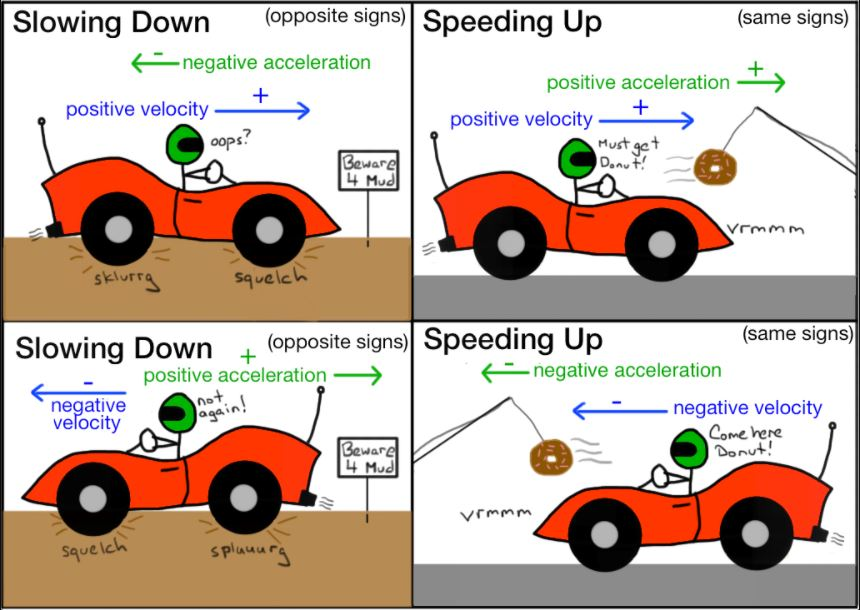
\includegraphics[width=0.6\textwidth]{images/fig4.JPG}}
			\caption{An explanation of acceleration.}
			\label{fig:acceleration}
		\end{center}
	\end{figure}
\end{itemize}

\subsection{Related Rates}
Related rates involve problems which involve two quantities that are changing at the same time. Given that the two rates are related, we can figure out how fast one of them is changing based on how fast the other is changing. This is usually done by implicitly differentiating a relation equation with respect to time, $t$.

\noindent \textbf{Examples:}
\begin{enumerate}
	\item Given the equation: $\frac{x}{y} = 9$, and $\frac{dy}{dt} = -\frac{2}{3}$, find $\frac{dx}{dt}$ when $x = 3$.

	To begin, implicitly differentiate the given equation $\frac{x}{y} = 9$ with respect to $t$:
	\begin{align*}
		\frac{x}{y} &= 9 \\[5pt]
		\frac{y \cdot \frac{dx}{dt} - x \cdot \frac{dy}{dt}}{y^2} &= 0 \\[5pt]
		y \cdot \frac{dx}{dt} - x \cdot \frac{dy}{dt} &= 0.
	\end{align*}

	In this new equation, there are two unknowns: $\frac{dx}{dt}$ and $y$. To solve for $\frac{dx}{dt}$, we first have to solve for $y$:
	\begin{align*}
		\frac{x}{y} &= 9 \\[5pt]
		y &= \frac{x}{9} \\[5pt]
		y &= \frac{3}{9} \\[5pt]
		y &= \frac{1}{3}
	\end{align*}

	Finally, solving for $\frac{dx}{dt}$:
	\begin{align*}
		y \cdot \frac{dx}{dt} - x \cdot \frac{dy}{dt} &= 0 \\[5pt]
		\frac{dx}{dt} &= \frac{x \cdot \frac{dy}{dt}}{y} \\[5pt]
		\frac{dx}{dt} &= \frac{3 \cdot \left( -\frac{2}{3} \right)}{\frac{1}{3}} \\[5pt]
		\frac{dx}{dt} &= -6
	\end{align*}

	\item The surface area of a sphere is increasing at a rate of $14 \pi$ square meters per hour. At a certain instant, the surface area is $36 \pi$ square meters. What is the rate of change of the volume of the sphere at that instant?

	First, list out relevant equations, and implicitly differentiate them with respect to time:
	\begin{itemize}
		\item Surface area, $SA$, of a sphere with radius $r$:
		\begin{align*}
			SA &= 4 \pi r^2 \\
			\frac{dSA}{dt} &= 8 \pi r \cdot \frac{dr}{dt}.
		\end{align*}

		\item Volume, $V$, of a sphere with radius $r$:
		\begin{align*}
			V &= \frac{4}{3} \pi r^3 \\[5pt]
			\frac{dV}{dt} &= 4 \pi r^2 \cdot \frac{dr}{dt}.
		\end{align*}
	\end{itemize}

	Within these four equations, there are several unknowns:
	\begin{itemize}
		\item The radius of the sphere, $r$.
		\item The rate of change of radius, $\frac{dr}{dt}$.
		\item The rate of change of volume, $\frac{dV}{dt}$.
	\end{itemize}

	Solving for $r$:
	\begin{align*}
		SA &= 4 \pi r^2 \\
		r^2 &= \frac{SA}{4 \pi} \\[5pt]
		r &= \sqrt{\frac{SA}{4 \pi}} \\[5pt]
		r &= \sqrt{\frac{36 \pi}{4 \pi}} \\[5pt]
		r &= 3
	\end{align*}

	Solving for $\frac{dr}{dt}$:
	\begin{align*}
		\frac{dSA}{dt} &= 8 \pi r \cdot \frac{dr}{dt} \\[5pt]
		\frac{dr}{dt} &= \frac{\frac{dSA}{dt}}{8 \pi r} \\[5pt]
		\frac{dr}{dt} &= \frac{14 \pi}{8 \pi \cdot 3} \\[5pt]
		\frac{dr}{dt} &= \frac{7}{12}
	\end{align*}

	Finally, solving for $\frac{dV}{dt}$:
	\begin{align*}
		\frac{dV}{dt} &= 4 \pi r^2 \cdot \frac{dr}{dt} \\[5pt]
		\frac{dV}{dt} &= 4 \pi \cdot 3^2 \cdot \frac{7}{12} \\[5pt]
		\frac{dV}{dt} &= 21 \pi
	\end{align*}

	Therefore, at this instance in time, the volume of the sphere is changing by $21 \pi$ meters cubed.
\end{enumerate}

\subsection{Local Linearity and Approximation}
Local linearity is the graphical representation of a derivative. By zooming in really close to a function that is differentiable on all points in its domain, it would eventually become a straight line. It is much easier to work with this straight line as a slope for approximating other values.

Given a function $f(x)$, the equation of the tangent line at a point where $x = a$ is given below. Notice that this equation resembles the point-slope form equation, $y = m(x - x_1) - y_1$. The slope, $m$, is the derivative at point $a$, $f'(a)$.
\[ y = f'(a) (x - a) + f(a) \]

This can be useful in approximating values on a graph that are close another, known value. For example, in Figure \ref{fig:linearity}, there is a graph with function $f(x) = \sqrt{x}$. The value of point $A$ is $\sqrt{0.25} = 0.5$. However, the point $B$ is at $\sqrt{0.3}$, which is harder to calculate. However, it can be observed that the tangent line at point $A$ comes really close to point $B$, so we can use local linearity to approximate the value of $B$.

\begin{figure}[H]
	\begin{center}
		\frame{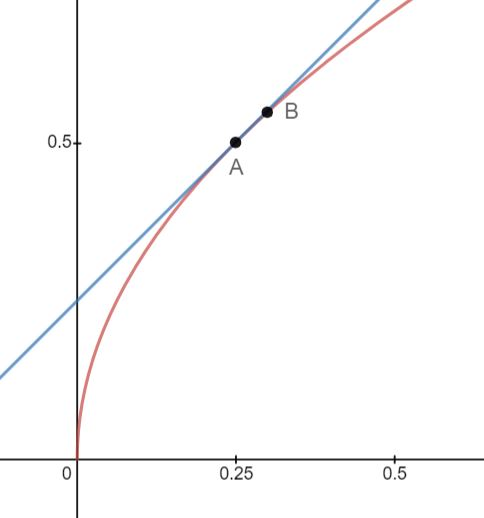
\includegraphics[width=0.4\textwidth]{images/fig5.JPG}}
		\caption{A demonstration of local linearity.}
		\label{fig:linearity}
	\end{center}
\end{figure}

The first step is to find the value of the slope at point $A$. This can be done by finding the value of the derivative at $x_A = 0.25$, or $f'(0.25)$.
\begin{align*}
	f(x) &= \sqrt{x} \\
	f'(x) &= \frac{1}{2} \cdot x^{-\frac{1}{2}} \\[5pt]
	f'(x) &= \frac{1}{2 \sqrt{x}} \\[5pt]
	f'(0.25) &= 1
\end{align*}

With this, we can plug in all required values into the local linearity line equation to get the equation of the tangent at point $A$.
\begin{align*}
	y &= f'(0.25) (x - 0.25) + f(0.25) \\
	y &= 1 (x - 0.25) + \sqrt{0.25} \\
	y &= x + 0.25
\end{align*}

Finally, to find the $y$ value of point $B$, substitute in the $x$ value of point $B$ into the above equation.
\begin{align*}
	y_B &= x_B + 0.25 \\
	y_B &= 0.3 + 0.25 \\
	y_B &= 0.55
\end{align*}

Therefore, point $B$ is located at approximately $(0.3, 0.55)$. Using a calculator reveals that the actual value of $B$ is $(0.3, 0.547)$, which is really close to the approximation.

\subsection{L'Hopital's Rule}
L'Hopital's rule allows the evaluation of limits in indeterminate forms. It states the following:
\begin{gather*}
	\text{if} \\
	\lim_{x \to c} \frac{f(x)}{g(x)} = \frac{0}{0} \quad \text{or} \quad \lim_{x \to c} \frac{f(x)}{g(x)} = \frac{\pm \infty}{\pm \infty} \\
	\text{then} \\
	\lim_{x \to c} \frac{f(x)}{g(x)} = \lim_{x \to c} \frac{f'(x)}{g'(x)}.
\end{gather*}

Note that l'Hopital's rule only applies if direct substitution of the limit evaluates to an indeterminate form. That is, if direct substitution gives a definite value, l'Hopital's rule will not work.

\noindent \textbf{Examples:}

\begin{enumerate}
	\item Find the value of $\lim \limits_{x \to 0} \frac{\sin x}{x}$.

	Direct substitution results in indeterminate form:
	\[ \lim_{x \to 0} \frac{\sin x}{x} = \frac{\sin 0}{0} = \frac{0}{0}. \]

	Using l'Hopital's rule, take the derivative of the numerator and denominator, separately. Then, reevaluate the limit:
	\begin{align*}
		\lim_{x \to 0} \frac{\sin x}{x} &= \lim_{x \to 0} \frac{\cos x}{1} \\[5pt]
		&= \frac{\cos 0}{1} \\[5pt]
		\lim_{x \to 0} \frac{\sin x}{x} &= 1.
	\end{align*}

	\item Find the value of $\lim \limits_{x \to \infty} \frac{e^x}{x^2}$.

	Direct substitution results in indeterminate form:
	\[ \lim_{x \to \infty} \frac{e^x}{x^2} = \frac{e^\infty}{\infty^2} = \frac{\infty}{\infty}. \]

	As with before, use l'Hopital's rule to take the derivative of the numerator and denominator. Then, reevaluate the limit:
	\[ \lim_{x \to \infty} \frac{e^x}{x^2} = \lim_{x \to \infty} \frac{e^x}{2x}. \]

	However, this limit still results in indeterminate form:
	\[ \lim_{x \to \infty} \frac{e^x}{2x} = \frac{e^\infty}{2 \cdot \infty} = \frac{\infty}{\infty}. \]

	Simply apply l'Hopital's rule again, then reevaluate the limit:
	\begin{align*}
		\lim_{x \to \infty} \frac{e^x}{2x} &= \lim_{x \to \infty} \frac{e^x}{2} \\[5pt]
		&= \frac{\infty}{2} \\[5pt]
		\lim_{x \to \infty} \frac{e^x}{2x} &= \infty.
	\end{align*}

	Therefore, the value of the original limit is also $\infty$.
\end{enumerate}

\subsubsection{Other Indeterminate Forms}
L'Hopital's rule can also be used to find limits involving exponential functions $f(x)^{g(x)}$. When taking the limit, the functions approach one of the following sets of values:

\begin{enumerate}
	\item $f(x) \to 0$ and $g(x) \to 0$
	\item $f(x) \to 1$ and $g(x) \to \infty$
	\item $f(x) \to \infty$ and $g(x) \to 0$
\end{enumerate}

Let $y = f(x)^{g(x)}$, and take the natural log of both sides. Rearrange and use l'Hopital's rule to solve the limit.
\begin{align*}
	y &= f(x)^{g(x)} \\
	\ln y &= g(x) \ln f(x) \\
	\lim_{x \to c} \ln y &= \lim_{x \to c} g(x) \ln f(x)
\end{align*}

\noindent For example, find the limit $\lim \limits_{x \to 0^+} x^x$.
\begin{align*}
	y &= x^x \\
	\ln y &= x \ln x \\
	\lim_{x \to 0^+} \ln y &= \lim_{x \to 0^+} x \ln x
\end{align*}

\noindent An attempt at direct substitution on the right-hand side results in an unfamiliar indeterminate form, $0 \times (- \infty)$. To solve this, rearrange the right-hand side to involve a fraction.
\[ \lim_{x \to 0^+} \ln y = \lim_{x \to 0^+} \frac{\ln x}{\frac{1}{x}}. \]

\noindent Now, direct substitution results in a workable indeterminate form:
\[ \lim_{x \to 0^+} \frac{\ln x}{\frac{1}{x}} = -\frac{\infty}{\infty}. \]

\noindent We can apply l'Hopital's rule again to solve this limit:
\begin{align*}
	\lim_{x \to 0^+} \ln y &= \lim_{x \to 0^+} \frac{\ln x}{\frac{1}{x}} \\[5pt]
	&= \lim_{x \to 0^+} \frac{\frac{1}{x}}{-\frac{1}{x^2}} \\[5pt]
	&= \lim_{x \to 0^+} -x \\
	\lim_{x \to 0^+} \ln y &= 0
\end{align*}

\noindent Finally, substitute this back into the original equation to find the limit $\lim \limits_{x \to 0^+} x^x$:
\begin{align*}
	\lim_{x \to 0^+} x^x &= \lim_{x \to 0^+} y \\
	&= \lim_{x \to 0^+} e^{\ln y} \\
	&= e^{\left( \lim \limits_{x \to 0^+} \ln y \right)} \\
	&= e^0 \\
	\lim_{x \to 0^+} x^x &= 1
\end{align*}

\noindent Note that in the step involving moving the limit operator inside the exponent:
\[ \lim_{x \to 0^+} e^{\ln y} = e^{\left( \lim \limits_{x \to 0^+} \ln y \right)}, \]
this is justified by the continuity of the function $e^x$. That is, $e^x$ is continuous everywhere including at $\lim \limits_{x \to 0^+} \ln y$, allowing the movement of the limit.

\subsection{Mean Value Theorem}
The mean value theorem states that for any arc between two endpoints on a graph, there will be a point whose tangent line is parallel to the secant line between the two endpoints.

\begin{figure}[H]
	\centering
	\frame{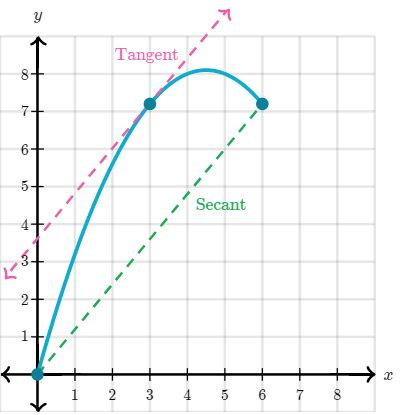
\includegraphics[width=0.4\textwidth]{images/fig6.JPG}}
	\caption{The mean value theorem.}
	\label{fig:mean_value_theorem}
\end{figure}

More precisely, given a \textit{continuous and differentiable} function $f(x)$ in the interval $[a, b]$, there exists a value $x = c, \; c \in [a, b]$ such that $f'(c)$ is equal to the average rate of change over $[a, b]$.
\[ f'(c) = \frac{f(b) - f(a)}{b - a}. \]

\subsection{Extreme Value Theorem}
If $f(x)$ is a continuous function over the closed interval $[a, b]$, then there exists a maximum and minimum value of $f(x)$. More formally, there much exist numbers $c$ and $d$ in $[a, b]$ such that $f(c) \leq f(x) \leq f(d)$ for all $x \in [a, b]$.

\subsection{First Derivative, Second Derivative and Candidates Tests}
The first derivative test, second derivative test, and candidates test are used together to find relative (or local) and absolute (or global) extrema in a function.

\subsubsection{Relative and Local Extrema}
A \textit{relative} maximum is a point on a graph where the function is the largest, relative to its immediate left and right. At this point, the function changes from increasing to decreasing. Similarly, a relative minimum is a point on a graph where the value of the function is the smallest, relative to its immediate left and right. At this point, the function changes from decreasing to increasing.

Points of extrema, such as a maximum or minimum, alongside points of inflection, are all categorized as critical points. Such points occur when the first derivative of the function is $0$ or undefined. Therefore, we can use the \textbf{first derivative test} to find extrema. For example, find the relative extremum of $f(x) = \frac{x^2}{x - 1}$.
\begin{align*}
	f(x) &= \frac{x^2}{x - 1} \\[5pt]
	f'(x) &= \frac{x^2 - 2x}{(x - 1)^2}
\end{align*}

\noindent The critical points occur at when $f'(x)$ is $0$ or undefined.
\begin{table}[H]
	\centering
	\begin{tabular}{|c|c|}
		\hline
		$x$ & $f'(x)$ \\
		\hline \hline
		$0, 2$ & $0$ \\
		\hline
		$1$ & undefined \\
		\hline
	\end{tabular}
\end{table}

\noindent Next, test the intervals between the critical points to see whether they are at a maximum, minimum, or point of inflection. This can be done by testing to see if the function is increasing ($f'(x) > 0$), or decreasing ($f'(x) < 0$) at each interval. Simply pick a random number in the interval and see if it is positive or negative.
\begin{table}[H]
	\centering
	\begin{tabular}{|c|c|c|}
		\hline
		Interval & $f'(x)$ & Slope of $f(x)$ \\
		\hline \hline
		$(-\infty, 0)$ & $+$ & $\nearrow$ \\
		\hline
		$(0, 1)$ & $-$ & $\searrow$ \\
		\hline
		$(1, 2)$ & $-$ & $\searrow$ \\
		\hline
		$(2, \infty)$ & $+$ & $\nearrow$ \\
		\hline
	\end{tabular}
\end{table}

\noindent At $x = 0$, $f'(x)$ switches from positive to negative, so $f(x)$ has a relative maximum. Similarly, at $x = 2$, $f'(x)$ switches from negative to positive, so $f(x)$ has a relative minimum. The sign of $f'(x)$ does not change at $x = 1$, so $f(x)$ experiences neither a relative maximum nor minimum, but rather a point of inflection (discussed in \ref{sec:concavity}).

An alternative, easier method for determining the nature of a critical point is the \textbf{second derivative test}. The second derivative is the change in the first derivative. Therefore, the sign of the second derivative determines whether the slope of the function is increasing or decreasing (not positive or negative). Given a point where $f'(x) = 0$, then:
\[ f''(x) \begin{cases}
	> 0 \Rightarrow \text{minimum point at } x \\
	< 0 \Rightarrow \text{maximum point at } x \\
	= 0 \Rightarrow \text{test is inconclusive}
\end{cases} \]

\subsubsection{Absolute and Global Extrema}
An \textit{absolute} extremum is a point where the function is at its largest or smallest across its entire domain. The method for finding absolute extrema is similar to that for finding relative ones, but with the extra consideration for the endpoints of the domain. For example, find the absolute extrema of $f(x) = x^3 + 2x^2$ for $-2 \leq x \leq 1$:

\noindent To begin, we can use the first derivative test to find the critical points:
\begin{align*}
	f(x) &= x^3 + 2x^2 \\
	f'(x) &= 3x^2 + 4x.
\end{align*}

\noindent Find the values for which $f'(x)$ is $0$ or undefined, the critical points:
\begin{table}[H]
	\centering
	\begin{tabular}{|c|c|}
		\hline
		$x$ & $f'(x)$ \\
		\hline \hline
		$-\frac{4}{3}, 0$ & $0$ \\
		\hline
	\end{tabular}
\end{table}

\noindent Determine the nature of the critical points using the second derivative test:
\begin{align*}
	f'(x) &= 3x^2 + 4x \\
	f''(x) &= 6x + 4
\end{align*}
\begin{table}[H]
	\centering
	\begin{tabular}{|c|c|}
		\hline
		$x$ & $f''(x)$ \\
		\hline \hline
		$-\frac{4}{3}$ & $-$ \\
		\hline
		$0$ & $+$ \\
		\hline
	\end{tabular}
\end{table}

\noindent This test concludes that $f(x)$ has a \textit{relative} maximum at $x = -\frac{4}{3}$ and a \textit{relative} minimum at $x = 0$. In order to find the global extrema, we have to consider the $y$ values of these points alongside $x = -2$ and $x = 1$, the endpoints of the closed interval.
\begin{table}[H]
	\centering
	\begin{tabular}{|c|c|}
		\hline
		$x$ & $y = f(x)$ \\
		\hline \hline
		$-2$ & $0$ \\
		\hline
		$-\frac{4}{3}$ & $\frac{32}{27} \approx 1.19$ \\
		\hline
		$0$ & $0$ \\
		\hline
		$1$ & $3$ \\
		\hline
	\end{tabular}
\end{table}

\noindent Therefore, it can be concluded that the absolute maximum of $f(x)$ is at $x = 1$. The $y$ values for $x = -2$ and $x = 0$ are the same, so both are absolute minimums.

\subsubsection{Concavity and Points of Inflection}
\label{sec:concavity}
Concavity is the sign of curvature of a function. Parts of a graph can either be \textit{concave up} or \textit{concave down}. When the concavity is concave up, the first derivative is increasing, thus the second derivative is positive. Inversely, when the concavity is concave down, the first derivative is decreasing, thus the second derivative is negative.

Inflection points are where the concavity flips. At inflection points both the first and second derivatives are $0$. Furthermore, at points of inflection the sign of the second derivative changes.

\begin{figure}[H]
	\begin{center}
		\frame{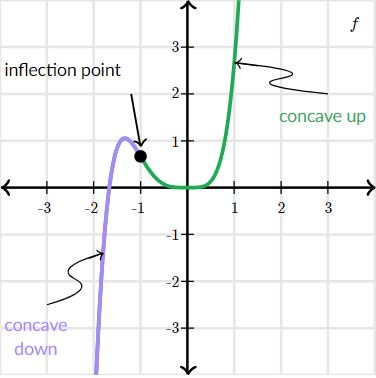
\includegraphics[width=0.4\textwidth]{fig8.JPG}}
		\caption{Concavity and points of inflection.}
		\label{fig:concavityinflection}
	\end{center}
\end{figure}

\subsection{Optimization Problems}
Optimization problems involve finding the largest or smallest something can be. This can be done by first find a function $f(x)$ to model the relationship between variables, then using $f'(x)$ to find the extrema.

\noindent \textbf{Examples:}
\begin{enumerate}
	\item Find the value of $x$ for which $y = 2x + 3$ is the closest to the origin.

	First, we can model the distance from a point $(x, y)$ to the origin, $(0, 0)$. This is given by:
	\[ D = \sqrt{x^2 + y^2}. \]

	Substitute in the given equation to get $D$ in terms of just $x$:
	\begin{align*}
		D &= \sqrt{x^2 + y^2} \\
		&= \sqrt{x^2 + (2x + 3)^2} \\
		D &= \sqrt{5x^2 + 12x + 9}.
	\end{align*}

	In order to find the minimum value of $D$, we can solve for the value of $x$ for which $\frac{dD}{dx} = 0$. First taking the derivative of $D$ with respect to $x$:
	\begin{align*}
		D &= \sqrt{5x^2 + 12x + 9} \\
		\frac{dD}{dx} &= \frac{5x + 6}{\sqrt{5x^2 + 12x + 9}}.
	\end{align*}

	Next finding the point where the derivative is $0$:
	\begin{align*}
		\frac{dD}{dx} &= 0 \\[5pt]
		\frac{5x + 6}{\sqrt{5x^2 + 12x + 9}} &= 0 \\[5pt]
		5x + 6 &= 0 \\
		x &= -\frac{6}{5}.
	\end{align*}

	We can use the second derivative test to determine whether $x = -\frac{6}{5}$ is a minimum value:
	\begin{align*}
		\frac{dD}{dx} &= \frac{5x + 6}{\sqrt{5x^2 + 12x + 9}} \\[5pt]
		\frac{d^2 D}{dx^2} &= \frac{9}{\left( 5x^2 + 12x + 9 \right)^{\frac{3}{2}}} \\[5pt]
		\frac{d^2 D}{dx^2} \Big|_{x = -\frac{6}{5}} &\approx 3.7.
	\end{align*}

	The second derivative is greater than $0$ at $x = -\frac{6}{5}$, so it can be concluded that this point is indeed a minimum point. Therefore, the function $y = 2x + 3$ will be closest to the origin at $x = -\frac{6}{5}$.

	\item Find the maximum product of two positive numbers whose sum if $300$.

	This question asks for a maximum $a \cdot b$ given $a + b = 300$. The first step if to represent the product in terms of a function of just one variable, $f(a)$.
	\begin{align*}
		b &= 300 - a \\
		ab &= a (300 - a) \\
		f(a) &= a (300 - a) \\
		f(a) &= 300a - a^2
	\end{align*}

	We can follow the same stems as the previous example to find the maximum of $f(a)$. First find the derivative of $f(a)$:
	\begin{align*}
		f(a) &= 300a - a^2 \\
		f'(a) &= 300 - 2a.
	\end{align*}

	Next, find the critical points:
	\begin{align*}
		f'(a) &= 0 \; \text{(or undefined)} \\
		300 - 2a &= 0 \\
		a &= 150.
	\end{align*}

	Use the second derivative test to validate that $a = 150$ is a maximum point:
	\begin{gather*}
		f'(a) = 300 - 2a \\
		f''(a) = -2 \\
		f''(a) < 0 \; \forall \; x \in \R.
	\end{gather*}

	Therefore, the value of $a$ that yields a maximum product is $150$. Now to find $b$:
	\begin{align*}
		a + b &= 300 \\
		150 + b &= 300 \\
		b &= 150.
	\end{align*}

	Finally, the two positive integers whose sum if $300$ and yield a maximum product are $150$ and $150$.

	\item We want to construct a cylindrical can with a bottom but no top that will have a volume of $30 \mathrm{cm^3}$. Determine the dimensions of the can that will minimize the amount of material needed to construct the can.

	First, we can list out the equations for the volume ($V$), and surface area ($SA$) of the specified can:
	\begin{gather*}
		V = \pi r^2 h \\
		SA = \pi r^2 + 2 \pi r h.
	\end{gather*}

	What we are trying to minimize in this question is the surface area. To begin, we can rewrite the $SA$ equation in terms of just one variable, $r$. First we can solve for $h$ in terms of $r$:
	\begin{align*}
		\pi r^2 h &= V \\
		\pi r^2 h &= 30 \\
		h &= \frac{30}{\pi r^2}.
	\end{align*}

	Next, rewrite the equation for $SA$ as a function of $r$:
	\begin{align*}
		SA &= \pi r^2 + 2 \pi r h \\
		SA(r) &= \pi r^2 + 2 \pi r \cdot \frac{30}{\pi r^2} \\[5pt]
		SA(r) &= \pi r^2 + \frac{60}{r}.
	\end{align*}

	Take the derivative of $SA(r)$:
	\begin{align*}
		SA(r) &= \pi r^2 + \frac{60}{r} \\[5pt]
		SA'(r) &= 2 \pi r - \frac{60}{r^2}.
	\end{align*}

	Find critical points:
	\begin{align*}
		SA'(r) &= 0 \\
		2 \pi r - \frac{60}{r^2} &= 0 \\
		2 \pi r^3 - 60 &= 0 \\
		r^3 &= \frac{30}{\pi} \\
		r &= \sqrt[3]{\frac{30}{\pi}}.
	\end{align*}

	Furthermore, $SA'(r)$ would be undefined at $r = 0$. However, the radius of a cylinder can not be $0$, so this would not actually be a valid critical point. We can use the second derivative test to validate the critical point $r = \sqrt[3]{\frac{30}{\pi}}$:
	\begin{gather*}
		SA''(r) = 2 \pi + \frac{120}{r^3} \\[5pt]
		SA'' \left( \sqrt[3]{\frac{30}{\pi}} \right) > 0
	\end{gather*}

	Therefore, $r = \sqrt[3]{\frac{30}{\pi}}$ would yield the least material used for the cylinder. Going back to solve for $h$:
	\begin{align*}
		h &= \frac{30}{\pi r^2} \\
		h &\approx 2.12.
	\end{align*}
\end{enumerate}

\subsection{Behaviors of Implicit Relations}
Implicit relations are equations that can not the rewritten to have one variable in terms of the other. They can be useful in solving for unknown values or line equations. When working with implicit relations and their derivatives, the key takeaway is that variables in the original equation and higher derivatives can be substituted both ways.

\noindent \textbf{Examples:}
\begin{enumerate}
	\item Consider the curve given by $x^3 + xy = -2$. It can be shown that $\frac{dy}{dx} = \frac{-3x^2 - y}{x}$. Find the point where the tangent line of the curve is horizontal.

	The tangent line of a curve is horizontal when its derivative is $0$. That is:
	\begin{align*}
		\frac{dy}{dx} &= 0 \\[5pt]
		\frac{-3x^2 - y}{x} &= 0 \\[5pt]
		3x^2 + y &= 0 , \; x \neq 0
	\end{align*}

	This equation along with the equation of the original curve provides a system of equations that can be solved:
	\[ \begin{cases}
		x^3 + xy = -2 \\
		3x^2 + y = 0 , \; x \neq 0
	\end{cases} \]

	Solving this would give the values $x = 1$ and $y = -3$. Therefore, at the point $(1, -3)$, the slope of the tangent line is $0$ and thus horizontal.
\end{enumerate}

\section{Integration and Accumulation of Change}
The accumulation of change is the net change of a quantity. This is not the same as simply the quantity. The accumulation of change takes into consideration time, and thus is the quantity over a specified time period. There may be a change in quantity before or after the specified time period, but that is not considered.

\subsection{Riemann Sums}
The Riemann sum is a method used to approximate the area under a curve. It splits up the area into several rectangles of equal width, whose heights match up with the function. The sum of the area of the rectangles would provide an approximation of the area.

The accuracy of the approximation can be improved by increasing the number of rectangles. This is done by decreasing $\Delta x$, the width of each rectangle.

\subsubsection{Types of Riemann Sums}
There are four main types of Riemann sums. Depending on the type of Riemann sum used, there may be either an over or under approximation of the actual area under the curve.
\begin{itemize}
	\item \textbf{Left Riemann Sum:} line up the left side of the rectangle with the curve of the function.
	\begin{figure}[H]
		\centering
		\frame{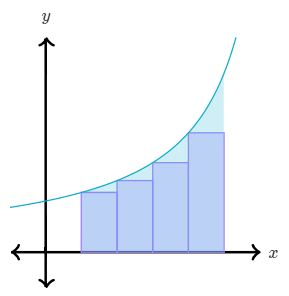
\includegraphics[width=0.4\textwidth]{images/fig9.JPG}}
		\caption{Left Riemann Sum.}
	\end{figure}

	\item \textbf{Right Riemann Sum:} line up the right side of the rectangle with the curve of the function.
	\begin{figure}[H]
		\centering
		\frame{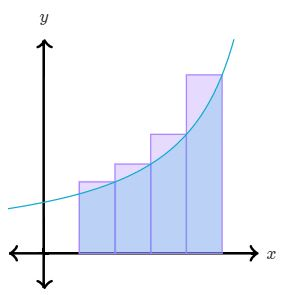
\includegraphics[width=0.4\textwidth]{images/fig10.JPG}}
		\caption{Right Riemann Sum.}
	\end{figure}

	\item \textbf{Midpoint Riemann Sum:} line up the middle of the rectangle with the curve of the function.
	\begin{figure}[H]
		\centering
		\frame{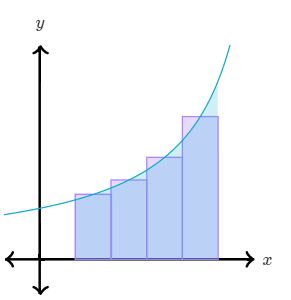
\includegraphics[width=0.4\textwidth]{images/fig11.JPG}}
		\caption{Midpoint Riemann Sum.}
	\end{figure}

	\item \textbf{Trapezoidal Sum:} uses trapezoids of equal height instead of rectangles to provide a better approximation of the area under the curve. The two bases of the trapezoid touch the curve of the function.
	\begin{figure}[H]
		\centering
		\frame{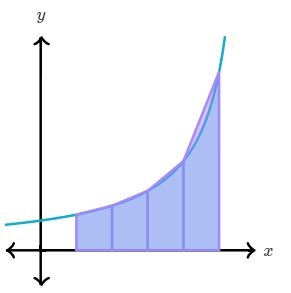
\includegraphics[width=0.4\textwidth]{images/fig12.JPG}}
		\caption{Trapezoidal Sum.}
	\end{figure}
\end{itemize}

\subsubsection{Reimann Sum in Summation Notation}
We want to approximate a function $f(x)$ using a Riemann sum over the interval $[a, b]$ with $n$ rectangles of equal width. We can define the width of each rectangle as ${\Delta x = \frac{b - a}{n}}$.

With \textit{left} Riemann sums, the rectangles can be labelled $i = 0$ through $i = n - 1$. The $i$-th rectangle will have its bottom left corner at an $x$ value of $a + \Delta x \cdot i$. Thus, the height of the $i$-th rectangle will be $f(a + \Delta x \cdot i)$. Therefore, the Riemann sum will be:
\[ \sum_{i = 0}^{n - 1} \Delta x \cdot f(a + \Delta x \cdot i). \]

With \textit{right} Riemann sums, the rectangles can be labelled $i = 1$ through $i = n$. The $i$-th rectangle will have its bottom right corner at an $x$ value of $a + \Delta x \cdot i$. Thus, the height of the $i$-th rectangle will be $f(a + \Delta x \cdot i)$. Therefore, the Riemann sum will be:
\[ \sum_{i = 1}^n \Delta x \cdot f(a + \Delta x \cdot i). \]

The summation notation for the midpoint Riemann sum and trapezoidal sum can be derived in similar fashions. The notation for a midpoint sum is:
\[ \sum_{i = 0}^{n - 1} \Delta x \cdot f \left( a + \Delta x \cdot \left( i + \frac{1}{2} \right) \right). \]

\noindent And the notation for a trapezoidal sum is:
\[ \sum_{i = 0}^{n - 1} \Delta x \cdot \frac{1}{2} \left[ f(a + \Delta x \cdot i) + f(a + \Delta x \cdot (i + 1)) \right]. \]

\subsection{Definite Integrals}
As the width of each rectangle, $\Delta x$, gets smaller and smaller, we are able to get an increasingly better approximation of the area under the curve. However, it is impossible to calculate the exact area under a curve using a finite number of rectangles.

For a better approximation, we can use an infinite number of rectangles, each with an infinitely small width. That is, $\Delta x$ approaches $0$. This is called a definite integral, and it can find the exact area of an interval under a curve. The notation for a definite integral over the interval $[a, b]$ of a function $f(x)$ is:
\[ \int_a^b f(x) \; dx. \]

\subsubsection{Definite Integral as a Riemann Sum}
The notation for a definite integral is quite similar to the Riemann sum. The height of each rectangle is given by $f(x)$, and the infinitely small width is given by $dx$. It's the same as:
\[ \lim_{n \to \infty} \sum_{i = 1}^n f(a + \Delta x \cdot i) \cdot \Delta x. \]

Any definite integral can be written as a Riemann sum. For example, write the following definite integral as a Riemann sum:
\[ \int_\pi^{2 \pi} \sin(x) \; dx. \]

\noindent First find $\Delta x$:
\begin{align*}
	\Delta x &= \frac{b - a}{n} \\[5pt]
	&= \frac{2 \pi - \pi}{n} \\[5pt]
	\Delta x &= \frac{\pi}{n}.
\end{align*}

\noindent Putting everything together:
\begin{gather*}
	\int_a^b f(x) \; dx = \lim_{n \to \infty} \sum_{i = 1}^n f(a + \Delta x \cdot i) \cdot \Delta x \\[5pt]
	\int_\pi^{2 \pi} \sin(x) \; dx = \lim_{n \to \infty} \sum_{i = 1}^n \sin \left( \pi + \frac{\pi}{n} \cdot i \right) \cdot \frac{\pi}{n} \\[5pt]
	\int_\pi^{2 \pi} \sin(x) \; dx = \lim_{n \to \infty} \sum_{i = 1}^n \sin \left( \pi + \frac{\pi i}{n} \right) \cdot \frac{\pi}{n}
\end{gather*}

\subsection{The Fundamental Theorem of Calculus}
We are given a function $f(x)$ that is continuous over the interval $[a, b]$. Let:
\[ F(x) = \int_a^x f(t) \; dt. \]

Recalling the notation for a definite integral, it is observed that $F(x)$ is the area under $f(x)$ from $a$ to $x$. $F(x)$ is the antiderivative of $f(x)$, and inversely, $f(x)$ is the derivative of $F(x)$. This allows us to solve for the area under a curve using antidifferentiation.
\[ \int_a^b f(x) \; dx = F(b) - F(a). \]

\subsection{Antiderivatives and Integration Techniques}
Antiderivatives are the reverse operation of a derivative. They are how to get from $f'(x)$ to $f(x)$. The symbol for an antiderivative is the integral symbol, without the bounds for a definite integral.

It is important to add a constant (usually represented by $C$), to the end of all antiderivative. Recall that the derivative of a constant is $0$. Thus, by adding a constant to the antiderivative, we consider the possibility of there being a constant term in $f(x)$.

\subsubsection{Reverse Power Rule}
\begin{gather*}
	\int x^n \; dx = \frac{x^{n + 1}}{n + 1} + C \\[5pt]
	\int \sqrt[m]{x^n} \; dx = \int x^{\frac{n}{m}} \; dx = \frac{x^{\frac{n}{m} + 1}}{\frac{n}{m} + 1} + C
\end{gather*}

\noindent This rule also applies to constants:
\begin{align*}
	\int A \; dx &= \int A x^0 \; dx \\
	&= \frac{A x^1}{1} + C \\[5pt]
	\int A \; dx &= Ax + C.
\end{align*}

\noindent The one exception to this rule is the antiderivative of $\frac{1}{x}$ or $x^{-1}$. Note the absolute value for the log:
\[ \int \frac{1}{x} \; dx = \ln |x| + C. \]

\subsubsection{Sum Rule of Integration}
\[ \int f(x) + g(x) \; dx = \int f(x) \; dx + \int g(x) \; dx \]

\subsubsection{Exponential Functions}
\begin{gather*}
	\int a^x \; dx = \frac{a^x}{\ln a} + C \\[5pt]
	\int e^x \; dx = e^x + C
\end{gather*}

\subsubsection{Basic Trigonometric Functions}
\begin{align*}
	\int \sin(x) \; dx &= -\cos(x) + C \\[5pt]
	\int \cos(x) \; dx &= \sin(x) + C \\[5pt]
	\int \sec^2(x) \; dx &= \tan(x) + C \\[5pt]
	\int \csc^2(x) \; dx &= -\cot(x) + C \\[5pt]
	\int \sec(x) \tan(x) \; dx &= \sec(x) + C \\[5pt]
	\int \csc(x) \cot(x) \; dx &= -\csc(x) + C
\end{align*}

\subsubsection{Special Case Trigonometric Functions}
These integrals may look messy, but come often come in handy.
\begin{align*}
	\int \frac{1}{\sqrt{a^2 - x^2}} \; dx &= \arcsin \left( \frac{x}{a} \right) + C \\[5pt]
	\int \frac{1}{\sqrt{a^2 - (bx)^2}} \; dx &= \frac{1}{b} \cdot \arcsin \left( \frac{bx}{a} \right) + C \\[5pt]
	\int \frac{1}{a^2 + x^2} \; dx &= \frac{1}{a} \cdot \arctan \left( \frac{x}{a} \right) + C \\[5pt]
	\int \frac{1}{a^2 + (bx)^2} \; dx &= \frac{1}{ab} \cdot \arctan \left( \frac{bx}{a} \right) + C
\end{align*}

\subsubsection{Integration by Parts}
Integration by parts is used to find the antiderivative of the product of functions. It is also referred to as the reverse power rule. The formula is:
\[ \int f(x) g'(x) \; dx = f(x) g(x) - \int f'(x) g(x) \; dx. \]

A tip for this technique is to have $f(x)$ be an easily differentiable function, while $g'(x)$ should be easily integrated. For example, integrate the following:
\[ \int x \cos x \; dx. \]

\noindent Let $f(x) = x$ and $g'(x) = \cos x$. This is because the derivative of $f(x)$ cancels out nicely to $1$, and the antiderivative of $g(x)$ doesn't get too complicated either. Thus, $f'(x) = 1$ and $g(x) = \sin x$. Substitute everything into the formula:
\begin{align*}
	\int x \cos x \; dx &= x \sin x - \int 1 \cdot \sin x \; dx \\[5pt]
	&= x \sin x - (-\cos x) + C \\
	\int x \cos x \; dx &= x \sin x + \cos x + C.
\end{align*}

\noindent Here is another example, find the integral of the following:
\[ \int \ln x \; dx. \]

\noindent Let $f(x) = \ln x$ and $g'(x) = 1$. Therefore, $f'(x) = \frac{1}{x}$ and $g(x) = x$. Substitute everything into the formula:
\begin{align*}
	\int \ln x \; dx &= x \ln x - \int \frac{1}{x} \cdot x \; dx \\[5pt]
	&= x \ln x - \int 1 \; dx \\[5pt]
	\int \ln x \; dx &= x \ln x - x + C.
\end{align*}

\subsubsection{U-Substitution}
Integration using u-substitution is also referred to as the reverse chain rule. It can be used when one part of a function resembles the derivative of another. For example, in the following integral:
\[ \int 2x \cos (x^2) \; dx, \]
notice that the derivative of $x^2$ is $2x$. Thus, we can let $u = x^2$, then implicitly differentiate:
\begin{align*}
	u &= x^2 \\
	\frac{d}{dx} (u) &= \frac{d}{dx} (x^2) \\[5pt]
	\frac{du}{dx} &= 2x.
\end{align*}

At this point, we can multiply both sides of the equation by $dx$. Note that while this step is usually considered unorthodox, it can help in this situation.
\[ 2x \; dx = du. \]

\noindent We can substitute this into the original integral to simplify it drastically:
\[ \int 2x \cos(x^2) \; dx = \int \cos(u) \; du. \]

\noindent Finally, solve the integral and substitute back $u = x^2$:
\begin{align*}
	\int 2x \cos(x^2) \; dx &= \int \cos(u) \; du \\[5pt]
	&= \sin(u) + C \\[5pt]
	\int 2x \cos(x^2) \; dx &= \sin(x^2) + C.
\end{align*}

Sometimes, more a bit manipulation is needed after u-substitution. For example, in the following integral:
\[ \int \sin(3x + 5) \; dx. \]

\noindent Let $u = 3x + 5$, and thus $du = 3 \; dx$. It may be useful to rearrange this equation to $dx = \frac{1}{3} \; du$, so we can directly substitute in $dx$. The integral then becomes:
\[ \int \frac{1}{3} \cdot \sin(u) \; du. \]

\noindent Solve and substitute back in $x$:
\begin{align*}
	\int \sin(3x + 5) \; dx &= \int \frac{1}{3} \cdot \sin(u) \; du \\[5pt]
	&= \frac{1}{3} \int \sin(u) \; du \\[5pt]
	&= -\frac{1}{3} \cos(u) + C \\[5pt]
	\int \sin(3x + 5) \; dx &= -\frac{\cos(3x + 5)}{3} + C.
\end{align*}

\subsubsection{Partial Fractions}
Partial fractions involve breaking up a fraction into the sum of several simpler ones for ease of integration. For example, integrate the following:
\[ \int \frac{2x + 3}{(x + 1)(x + 2)} \; dx. \]

The integrand is a big fraction that might get messy if we try to integrate directly. Rather, we notice that its denominator is made up of two smaller functions, and we can split up the large function according to the two separate denominators. Let $A$ and $B$ be the numerators of the two smaller functions. We write the following:
\begin{align*}
	\frac{2x + 3}{(x + 1)(x + 2)} &= \frac{A}{x + 1} + \frac{B}{x + 2} \\[5pt]
	\frac{2x + 3}{(x + 1)(x + 2)} &= \frac{A(x + 2) + B(x + 1)}{(x + 1)(x + 2)} \\[5pt]
	2x + 3 &= A(x + 2) + B(x + 1) \\
	&= Ax + 2A + Bx + B \\
	2x + 3 &= (A + B)x + 2A + B.
\end{align*}

\noindent By equating coefficients we get the following system, which can be solved:
\begin{gather*}
	\begin{cases}
		A + B = 2 \\
		2A + B = 3
	\end{cases} \\
	\therefore A = 1, B = 1
\end{gather*}

\noindent Returning to the original problem:
\begin{align*}
	\int \frac{2x + 3}{(x + 1)(x + 2)} \; dx &= \int \frac{1}{x + 1} + \frac{1}{x + 2} \; dx \\[5pt]
	&= \int \frac{1}{x + 1} \; dx + \int \frac{1}{x + 2} \; dx \\[5pt]
	\int \frac{2x + 3}{(x + 1)(x + 2)} \; dx &= \ln |x + 1| + \ln |x + 2| + C.
\end{align*}

\subsubsection{Other Integration Techniques}
\begin{itemize}
	\item \textbf{Long division:} when encountering a fraction with an equal degree numerator and denominator, divide the polynomials. This is most useful when methods like u-subsection do not work. For example:
	\[ \frac{2x + 7}{x + 3} = 2 + \frac{1}{x + 3}. \]

	\item \textbf{Completing the square:} when encountering a function that seems difficult to integrate. Completing the square may rearrange the function to resemble an easily integrable pattern. For example:
	\[ \int \frac{1}{6x^2 + 36x + 78} \; dx. \]

	There is no easy way to deal with the polynomial in the denominator. But by completing the square:
	\begin{align*}
		\frac{1}{6x^2 + 36x + 78} &= \frac{1}{6} \cdot \frac{1}{x^2 + 6x + 13} \\[5pt]
		\frac{1}{6x^2 + 36x + 78} &= \frac{1}{6} \cdot \frac{1}{(x + 3)^2 + 4},
	\end{align*}
	we notice that this now resembles a function that integrates into $\arctan$. Integrate as follows:
	\begin{align*}
		\int \frac{1}{6x^2 + 36x + 78} \; dx &= \int \frac{1}{6} \cdot \frac{1}{(x + 3)^2 + 4} \; dx \\[5pt]
		&= \frac{1}{6} \int \frac{1}{(x + 3)^2 + 4} \; dx \\[5pt]
		&= \frac{1}{6} \cdot \frac{1}{2} \arctan \left( \frac{x + 3}{2} \right) \\[5pt]
		\int \frac{1}{6x^2 + 36x + 78} \; dx &= \frac{1}{12} \arctan \left( \frac{x + 3}{2} \right).
	\end{align*}
\end{itemize}

\subsection{Solving Definite Integrals}
The method for solving definite integrals comes directly from the fundamental theorem of calculus. Recall:
\[ \int_a^b f(x) \; dx = F(b) - F(a), \]
where $F(x)$ is the antiderivative of $f(x)$. Usually the antiderivative would be written in the form:
\[ [F(x)]_a^b, \]
which just means $F(b) - F(a)$. Note that if $a = b$, then the value of the definite integral would be $0$:
\[ \int_a^a f(x) \; dx = 0. \]

\noindent \textbf{Examples:}
\begin{enumerate}
	\item Solve the following definite integral:
	\begin{align*}
		\int_{-1}^2 x^2 \; dx &= [2x]_{-1}^2 \\[5pt]
		&= 2 \cdot 2 - 2 \cdot (-1) \\
		\int_{-1}^2 x^2 \; dx &= 6.
	\end{align*}

	\item Find the area under the curve of $\frac{8}{x^2}$ from $x = e$ to $x = e^2$.

	This area can be modelled using a definite integral:
	\[ \int_e^{e^2} \frac{8}{x} \; dx. \]

	Solve the integral to find the area under the curve:
	\begin{align*}
		\int_e^{e^2} \frac{8}{x} \; dx &= 8 \int_e^{e^2} \frac{1}{x} \; dx \\[5pt]
		&= 8 [\ln x]_e^{e^2} \\
		&= 8 (\ln (e^2) - \ln (e)) \\
		\int_e^{e^2} \frac{8}{x} \; dx &= 8.
	\end{align*}
\end{enumerate}

\subsection{Improper Integrals}
Improper integrals are definite integrals that have one or both endpoints at infinity, or an integrand that approaches infinity. Such integrals can not be evaluated using a Riemann Sum.

One type of improper integral occurs when at least one of the endpoints is infinity. The endpoint can therefore be rewritten as a limit. For example:
\[ \int_1^\infty \frac{1}{x^2} \; dx = \lim_{a \to \infty} \int_1^a \frac{1}{x^2} \; dx. \]
Given that the limit of the integrand converges, or approaches a finite value, the definite integral can be evaluated as follows:
\begin{align*}
	\int_1^\infty \frac{1}{x^2} \; dx &= \left[ -\frac{1}{x} \right]_1^\infty \\[5pt]
	&= \lim_{a \to \infty} \left[ -\frac{1}{x} \right]_1^a \\[5pt]
	&= \lim_{a \to \infty} \left( -\frac{1}{1} - \left( -\frac{1}{a} \right) \right) \\[5pt]
	&= \lim_{a \to \infty} \left( -1 + \frac{1}{a} \right) \\[5pt]
	\int_1^\infty \frac{1}{x^2} \; dx &= -1
\end{align*}

The other type of improper integral occurs when the integrand evaluates to infinity or an undefined value at least one of the endpoints. As with before, the endpoint can be rewritten as a limit. For example:
\[ \int_0^5 \frac{1}{\sqrt{x}} \; dx = \lim_{a \to 0^+} \int_a^5 \frac{1}{\sqrt{x}} \; dx. \]
Such integrals can also be solved using limits:
\begin{align*}
	\int_0^5 \frac{1}{\sqrt{x}} \; dx &= \lim_{a \to 0^+} [2 \sqrt{x}]_a^5 \\[5pt]
	&= \lim_{a \to 0^+} (2 \sqrt{5} - 2 \sqrt{a}) \\
	\int_0^5 \frac{1}{\sqrt{x}} \; dx &= 2 \sqrt{5}.
\end{align*}

\section{Differential Equations}
Differential equations involve variables and their derivatives. Unlike algebraic equations which evaluate to numbers or values, differential equations evaluate to a function of class of (several) functions.

\subsection{Modelling Differential Equations}
When interpreting words to model differential equations, there a few keywords that should be looked out for. They are listed below:
\begin{itemize}
	\item \textbf{Proportional:} means that the rate of change of one variable is equal to some constant $k$ multiplied by the another variable.

	A habitat of prairie dogs can support at most $m$ dogs. The habitat's population, $p$, grows proportionally to the product of the current population and $m - p$.

	The population's rate of change can be modelled using:
	\[ \frac{dp}{dt} = kp(m - p). \]

	\item \textbf{Shrinks, decays, melts, decreases, etc.:} any word that suggests something is getting smaller, the rate of change of one variable would be negative proportional to another variable.

	A radioactive material decays at a rate proportional the current amount, $Q$, of the material.

	The amount of material can be modelled using:
	\[ \frac{dQ}{dt} = -kQ. \]

	\item \textbf{Inversely Proportional:}

	\item \textbf{Fraction of ... :}
\end{itemize}

\subsection{Slope Fields}

\subsection{Euler's Method Approximation}

\subsection{Separable Differential Equations}

\subsubsection{General Solutions}

\subsubsection{Particular Solutions}

\subsection{Homogeneous Differential Equations}

\subsection{Integrating Factor}

\subsection{Exponential Model Equations}

\subsection{Logistic Growth Model Equations}

\end{document}